\chapter{Results and Discussion}

\section{Experimental Setup}
The experiments follow the protocol of Chapter~4. After the inner join and the one-day lag, the data are divided chronologically into a training set (the first 70\% of days: \TrainDays{} trading days, \TrainRange{}), a validation set (the next 15\%: \ValDays{} days, \ValRange{}) and a test set (the final 15\%: \TestDays{} days, \TestRange{}). The test set contains \UpShareTest{} Up days, so a classifier that always predicts the majority class reaches an accuracy of \BaselineAcc{}. With \TestDays{} test days, the 95\% margin of error on an accuracy near one half is \MarginErr{} percentage points. All numbers below come from the experiment notebooks (file \texttt{results.csv}) and are inserted into the report by the script \texttt{make\_results\_table.py}, so that the text and the tables cannot disagree.

\section{Main Results}
Table~\ref{tab:results} reports test-set performance of all nine experiments (three models on three feature sets).

\begin{table}[!htbp]
\centering
\small
\setlength{\tabcolsep}{4pt}
\begin{tabular}{@{}llccccc@{}}
\toprule
Feature set & Model & Accuracy & Precision & Recall & F1 & ROC-AUC \\
\midrule
Numerical-only & Logistic Regression & 0.498 & 0.500 & 0.993 & 0.665 & 0.520 \\
 & Random Forest & 0.512 & 0.507 & 0.913 & 0.652 & 0.487 \\
 & XGBoost & 0.498 & 0.500 & 0.926 & 0.649 & 0.482 \\
\midrule
Sentiment-only & Logistic Regression & 0.505 & 0.503 & 0.973 & 0.664 & 0.524 \\
 & Random Forest & 0.502 & 0.502 & 0.779 & 0.611 & 0.520 \\
 & XGBoost & 0.478 & 0.482 & 0.550 & 0.514 & 0.500 \\
\midrule
Multimodal & Logistic Regression & 0.498 & 0.500 & 0.933 & 0.651 & \textbf{0.539} \\
 & Random Forest & 0.512 & 0.507 & 0.966 & 0.665 & 0.483 \\
 & XGBoost & 0.522 & 0.515 & 0.826 & 0.634 & 0.481 \\
\midrule
\multicolumn{2}{l}{Majority-class baseline} & 0.502 & -- & -- & -- & 0.500 \\
\bottomrule
\end{tabular}

\caption{Test-set performance of each model on each feature set.}
\label{tab:results}
\end{table}

The best-performing combination by ROC-AUC is \BestModel{} on the \BestFeatureSet{} feature set, with a ROC-AUC of \BestAUC{} and an accuracy of \BestAcc{}. The majority-class baseline is \BaselineAcc{}.

\subsection{What the numbers show}
\begin{itemize}
  \item \textbf{Accuracy is at the baseline.} The nine accuracies range from 47.8\% (sentiment-only XGBoost) to 52.2\% (multimodal XGBoost). Every value is within the margin of error of the 50.2\% baseline, so none of the models is distinguishable from always guessing the majority class.
  \item \textbf{ROC-AUC is close to 0.5.} The values range from 0.481 to 0.539. The highest, multimodal Logistic Regression at \BestAUC{}, is only about 0.04 above chance, and at \TestDays{} test days the sampling uncertainty of an AUC is of the order of $\pm0.06$, so even this value cannot be separated from chance with confidence.
  \item \textbf{Sentiment adds little.} The best multimodal AUC (\MMBestAUC{}) exceeds the best numerical-only AUC (\NumBestAUC{}) by \AUCDelta{}, which is well inside the sampling uncertainty. For Random Forest and XGBoost the multimodal AUC is in fact slightly lower than that of the Logistic Regression models, and sentiment-only features alone reach at most 0.524.
  \item \textbf{High recall is an artefact.} Recall for the Up class is 0.55 to 0.99 for all models, while precision stays near 0.50. The models predict Up on most days, and recall is high because most of the Up days are caught by chance, not because of skill. The confusion matrices in Figure~\ref{fig:cm} confirm this: for numerical-only Logistic Regression, 296 of 297 predictions are Up. Table~\ref{tab:bias} shows that the balanced accuracy of all models is close to 0.5.
  \item \textbf{Validation is not a reliable guide.} The cross-validated AUC on the training data is about 0.47 to 0.52 for all experiments, and the validation AUC varies from 0.455 to 0.580 (the highest, numerical-only Logistic Regression, falls to 0.520 on the test set). This instability is typical of a signal that is too weak to be measured reliably.
\end{itemize}

\section{Effect of the Feature Set}
The ablation compares the best ROC-AUC obtained with numerical features alone (\NumBestAUC) to the best obtained with the multimodal features (\MMBestAUC), a difference of \AUCDelta{}. Figure~\ref{fig:roc} shows the ROC curves of the three models for each feature set, and Figure~\ref{fig:featimp} shows which features the tree-based models rely on.

\begin{figure}[!htbp]
\centering
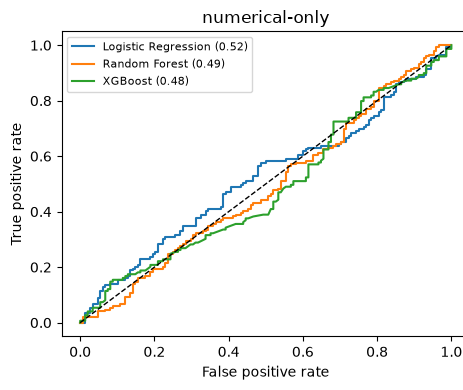
\includegraphics[width=0.49\textwidth]{figures/fig_roc_numerical.png}\hfill
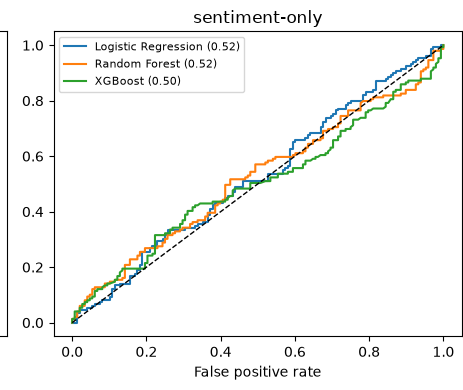
\includegraphics[width=0.49\textwidth]{figures/fig_roc_sentiment.png}\\[4pt]
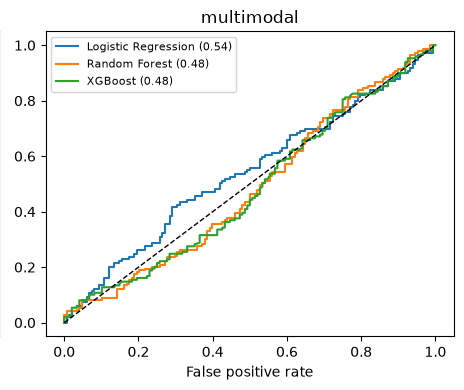
\includegraphics[width=0.49\textwidth]{figures/fig_roc_multimodal.png}
\caption{ROC curves on the test set for the three feature sets; the legend gives the ROC-AUC of each model and the dashed line is chance.}
\label{fig:roc}
\end{figure}

\begin{figure}[!htbp]
\centering
\maybefigure{fig_feature_importance.png}{0.98\textwidth}{6.5cm}{Feature importance of the multimodal Random Forest or XGBoost model, with sentiment features highlighted}
\caption{Feature importance in the multimodal models: absolute coefficient for Logistic Regression and impurity-based importance for Random Forest and XGBoost (\texttt{sent\_pos}, \texttt{sent\_neg}, \texttt{sent\_neu} correspond to the three daily sentiment means).}
\label{fig:featimp}
\end{figure}

\section{Confusion Matrices}
Accuracy alone does not reveal whether a model simply predicts one class most of the time. Figure~\ref{fig:cm} shows the confusion matrices of all nine experiments. Nearly all models predict Up on most days, so recall for Up is high and almost no Down day is identified correctly; the matrices make this visible.

\begin{figure}[!htbp]
\centering
\maybefigure{fig_confusion.png}{0.95\textwidth}{5.5cm}{Three confusion matrices side by side (numerical-only, sentiment-only, multimodal) for the best model of each set}
\caption{Confusion matrices of all nine experiments on the test set (rows: true class, columns: predicted class).}
\label{fig:cm}
\end{figure}

\section{Bias Towards the Up Class}
The high recall and F1-score of most models (Table~\ref{tab:results}) invite a misreading, so the share of Up predictions and the balanced accuracy were computed for every experiment (Table~\ref{tab:bias}). Balanced accuracy is the mean of the recall on Down days and the recall on Up days; a model without skill obtains 0.5 whatever its class bias. The test set contains 50.2\% Up days.

\begin{table}[!htbp]
\centering
\small
\begin{tabular}{@{}llccc@{}}
\toprule
Feature set & Model & Predicted Up & Accuracy & Balanced accuracy \\
\midrule
Numerical-only & Logistic Regression & 0.997 & 0.498 & 0.497 \\
 & Random Forest & 0.902 & 0.512 & 0.510 \\
 & XGBoost & 0.929 & 0.498 & 0.497 \\
\midrule
Sentiment-only & Logistic Regression & 0.970 & 0.505 & 0.503 \\
 & Random Forest & 0.778 & 0.502 & 0.501 \\
 & XGBoost & 0.572 & 0.478 & 0.478 \\
\midrule
Multimodal & Logistic Regression & 0.936 & 0.498 & 0.497 \\
 & Random Forest & 0.956 & 0.512 & 0.510 \\
 & XGBoost & 0.805 & 0.522 & 0.521 \\
\bottomrule
\end{tabular}
\caption{Share of test days predicted as Up, accuracy and balanced accuracy of the nine experiments.}
\label{tab:bias}
\end{table}

Eight of the nine models predict Up on more than three quarters of the days, and numerical-only Logistic Regression does so on 99.7\% of them. Their balanced accuracy lies between 0.478 and 0.521, that is, at the no-skill value of 0.5 within the sampling error. The F1-scores of about 0.65 are therefore a consequence of the Up bias and not evidence of skill: a classifier that always predicts Up has recall 1.0 and an F1-score of 0.67 on this test set.

\section{Demonstration Forecasts}
\label{sec:forecast}
Two forecasts were produced to show how the trained pipeline is used. They are demonstrations of the procedure, not evidence of skill: a single call is right with probability one half even for a coin flip.

\paragraph{Last day of the data set.} The multimodal model with the highest validation ROC-AUC is Logistic Regression ($C=0.01$, validation AUC 0.538). Refitted on the training and validation rows, it gives a probability of 0.517 that the market closes higher after 30 June 2016, that is, the prediction Up. The actual direction was Up. The probability is very close to 0.5, so the model expresses almost no confidence.

\paragraph{Current data.} The notebook \texttt{tomorrow.ipynb} downloads recent S\&P 500 prices and applies the numerical-only Logistic Regression ($C=0.01$), fitted on all 1,978 days of 2008 to 2016 (Section~\ref{sec:live}). The most recent close in the data downloaded was 7,561.67 on 13 November 2026, and the model gave a probability of 0.561 that the next trading day closes higher, that is, Up. For reference, the probabilities produced by the same model on the historical days range from 0.348 to 0.686 with a median of 0.540, so 0.561 is a weak, near-neutral signal. Because the model has no measured skill on the test period (Table~\ref{tab:bias}), this output must not be used as a trading signal. Sentiment is not part of this forecast because no current headline feed is available.

\section{How to Interpret the Results}
\label{sec:interpret}
The following reading guide applies regardless of the specific numbers obtained.
\begin{itemize}
  \item \textbf{Compare with the baseline first.} An accuracy equal to the majority-class share indicates that the model has learned nothing beyond the class balance. Only accuracy above baseline by more than the margin of error is evidence of skill.
  \item \textbf{Use ROC-AUC for ranking skill.} A ROC-AUC near 0.50 means the model's scores do not rank Up days above Down days. Values in the low 0.50s are typical for this task and are at the edge of what can be distinguished from noise on a test set of a few hundred days.
  \item \textbf{Judge the multimodal benefit by the difference.} If multimodal and numerical-only ROC-AUC differ by less than the sampling uncertainty, the honest conclusion is that sentiment did not demonstrably help; if multimodal is clearly higher, sentiment contributes complementary information.
  \item \textbf{Be suspicious of very high scores.} Next-day direction is close to unpredictable. Accuracy near 90\% or above would indicate leakage, as in the 100\% figure of the reviewed preprint, and would call for a check of the pipeline, not a celebration.
\end{itemize}

\section{Discussion}
\subsection{Why the signal is expected to be weak}
Several features of the problem limit what any model can achieve. The efficient market hypothesis predicts that public information is rapidly incorporated into prices. Daily index direction is the net effect of thousands of simultaneous events, and most of its variance is unrelated to the average sentiment of 25 headlines from a general world-news forum. The Reddit headlines are not specific to finance: many concern politics and conflicts, and FinBERT, trained on financial text, may assign confident sentiment to sentences outside its domain.

\subsection{Role of each model}
Logistic Regression has little capacity to overfit, so it is expected to be competitive with the more flexible models when the signal is weak. Random Forest and XGBoost can capture interactions but also fit noise; their depth limits and the walk-forward tuning are intended to restrain them. If the flexible models achieve a higher cross-validated AUC but not a higher test AUC, that is a sign of overfitting to the validation folds.

\subsection{Effect of the sentiment lag}
The one-day lag makes the design conservative. It guarantees that the sentiment used on day $t$ was available before the target day, but it may also discard a genuine same-day relationship, because headlines published in the morning could influence the same day's close. This design choice favours validity over apparent performance, and the lag can be set to zero as a sensitivity check (with the caveat that the result then depends on the unknown publication time).

\subsection{Limitations}
\begin{itemize}
  \item The test period is a single contiguous stretch of a rising market, so the results may not generalise to other regimes such as sharp declines.
  \item The text input is limited to Reddit headlines, which are crowd-curated and not guaranteed to be representative of financial news flow.
  \item The sentiment encoder is applied to headlines without fine-tuning on the target task.
  \item The study evaluates classification quality and not trading performance, so transaction costs and risk are not considered.
  \item With a few hundred test days, differences of a few percentage points are within sampling error.
\end{itemize}
